\documentclass[sigconf]{acmart}

\usepackage{color}
\usepackage{balance}
\usepackage{blindtext}
\usepackage{comment}
\usepackage{amsmath}
\usepackage{enumitem}
\usepackage{array}
\usepackage{graphicx}
\usepackage{subcaption}
\usepackage{tabularx}
\usepackage{ragged2e}
\usepackage{adjustbox}
\usepackage{multirow}
\usepackage{booktabs}
\usepackage{caption}
\usepackage{float}
\usepackage{url}
\usepackage{xspace}
\usepackage[newfloat]{minted}
\usepackage[english]{babel}



\newenvironment{code}{\captionsetup{type=listing}}{}
\SetupFloatingEnvironment{listing}{name=Listing}
\newcolumntype{P}[1]{>{\centering\arraybackslash}m{#1}}

% Copyright
\setcopyright{none}
%\setcopyright{acmcopyright}
%\setcopyright{acmlicensed}
% \setcopyright{rightsretained}
%\setcopyright{usgov}
%\setcopyright{usgovmixed}
%\setcopyright{cagov}
%\setcopyright{cagovmixed}

\setlength{\textfloatsep}{5pt}
\setlength{\intextsep}{5pt}
\newcommand{\namex}{\mbox{\sf Compass}}
\newcommand{\name}{\namex\xspace}
\newcommand{\Paragraph}[1]{~\vspace*{-0.8\baselineskip}\\{\bf #1}}
\DeclareMathOperator{\sen}{sen}
\newcommand{\Q}{\mathbb{Q}}
\newcommand{\alphastar}{\alpha^{*}}
\newcommand{\blue}[1]{{\color{blue} #1}}

\newcommand{\cb}[1]{{\color{blue} #1}}

%\newtheorem{definition}{Definition}
%\newtheorem{theorem}{Theorem}
%%\newtheorem{proof}{Proof}
%\newtheorem{lemma}{Lemma}
%\newtheorem{corollary}{Corollary}

\newcommand\Tstrut{\rule{0pt}{2.6ex}}       % "top" strut
\newcommand\Bstrut{\rule[-0.9ex]{0pt}{0pt}} % "bottom" strut
\newcommand{\TBstrut}{\Tstrut\Bstrut} % top&bottom struts

%\renewcommand{\algorithmicrequire}{\textbf{Input:}}
%\renewcommand{\algorithmicensure}{\textbf{Output:}}
\newcommand\floor[1]{\lfloor#1\rfloor}
\newcommand\ceil[1]{\lceil#1\rceil}
\newcommand\F{\widehat{F}}
\newcommand\be{\widehat{b}}

\newcommand{\pbex}{\mbox{\sf PBE}}
\newcommand{\pbe}{\pbex\xspace}
\newcommand{\pbeaX}{\mbox{\sf PBE-1}}
\newcommand{\pbea}{\pbeaX\xspace}
\newcommand{\pbebX}{\mbox{\sf PBE-2}}
\newcommand{\pbeb}{\pbebX\xspace}
\newcommand{\cmpbeaX}{\mbox{\sf CM-PBE-1}}
\newcommand{\cmpbea}{\cmpbeaX\xspace}
\newcommand{\cmpbebX}{\mbox{\sf CM-PBE-2}}
\newcommand{\cmpbeb}{\cmpbebX\xspace}
\newcommand{\cmpbex}{\mbox{\sf CM-PBE}}
\newcommand{\cmpbe}{\cmpbex\xspace}
\newcommand{\eps}{\varepsilon}


\newtheorem{informal}{Informal Problem}
\newtheorem*{formal}{Open Attribute Value Extraction}
\newcommand{\sysname}{{\sf OpenTag}\xspace}
%\newcommand{\softmax}{\operatornamewithlimits{softmax}}
%\newcommand{\argmax}{\operatornamewithlimits{argmax}}
\DeclareMathOperator{\softmax}{softmax}
\DeclareMathOperator{\argmax}{argmax}
\DeclareMathOperator{\argmin}{argmin}
\pagenumbering{arabic}
\setcounter{page}{1}

\newenvironment{pkl}{%
\begin{itemize}%
%\vspace{-\topsep}%
\setlength\itemsep{-0.5\parskip}%
\setlength\parsep{0in}%
}{%
%\vspace{-\topsep}%
\end{itemize}}

\newenvironment{des}{%
\begin{description}%
%\vspace{-\topsep}%
\setlength\itemsep{-0.5\parskip}%
\setlength\parsep{0in}%
}{%
%\vspace{-\topsep}%
\end{description}}


\newenvironment{enu}{%
\begin{enumerate}%
\vspace{-\topsep}%
\setlength\itemsep{-\parskip}%
\setlength\parsep{0in}%
}{%
\vspace{-\topsep}%
\end{enumerate}}



%Conference

\copyrightyear{2018}
\acmYear{2018}
%\setcopyright{none}
\acmConference{University of Utah}{}{ Salt Lake City, USA.}
%\acmPrice{15.00}
%\acmISBN{-}
%\acmDOI{-}


\setlength{\textfloatsep}{1pt}
\setlength{\intextsep}{7pt}
\setlength{\floatsep}{3pt}

\begin{document}
\title{ Social Media Data and its availability in Research }
% \titlenote{Produces the permission block, and
%   copyright information}
%\subtitle{}
%\subtitlenote{The full version of the author's guide is available as
%  \texttt{acmart.pdf} document}

\author{Debjyoti Paul}
\affiliation{%
    \institution{University of Utah}
}
\email{deb@cs.utah.edu}




% The default list of authors is too long for headers}
%\renewcommand{\shortauthors}{B. Trovato et al.}

% \begin{abstract}

\end{abstract}


%
% The code below should be generated by the tool at
% http://dl.acm.org/ccs.cfm
% Please copy and paste the code instead of the example below.
%
%\begin{CCSXML}
%<ccs2012>
% <concept>
%  <concept_id>10010520.10010553.10010562</concept_id>
%  <concept_desc>Computer systems organization~Embedded systems</concept_desc>
%  <concept_significance>500</concept_significance>
% </concept>
% <concept>
%  <concept_id>10010520.10010575.10010755</concept_id>
%  <concept_desc>Computer systems organization~Redundancy</concept_desc>
%  <concept_significance>300</concept_significance>
% </concept>
% <concept>
%  <concept_id>10010520.10010553.10010554</concept_id>
%  <concept_desc>Computer systems organization~Robotics</concept_desc>
%  <concept_significance>100</concept_significance>
% </concept>
% <concept>
%  <concept_id>10003033.10003083.10003095</concept_id>
%  <concept_desc>Networks~Network reliability</concept_desc>
%  <concept_significance>100</concept_significance>
% </concept>
%</ccs2012>
%\end{CCSXML}
%
%\ccsdesc[500]{Computer systems organization~Embedded systems}
%\ccsdesc[300]{Computer systems organization~Redundancy}
%\ccsdesc{Computer systems organization~Robotics}
%\ccsdesc[100]{Networks~Network reliability}
%
% We no longer use \terms command
%\terms{Theory}

%\keywords{ streaming data, bursty, data sketch, historical queries}


\maketitle

% \begin{abstract}

\end{abstract}

\section*{Overview}
\label{sec:overview}
The term {\em Social Media} gained widespread attention with the advent of Web 2.0 in the first decade of 20th century \cite{kaplan2010users}. Web 2.0 is also known as {\em participative} or {\em social web} that emphasize on user interaction and user generated content encouraging participatory culture. Before we jump into more details of social media, it would be wiser to define it.
The dynamic changes and continuous development of social media services makes it harder to define them, however most of the research work could be summarized it as follows.

\begin{definition}[Social Media]
Social media is an interactive computer mediated technological platform that facilitates the creation and sharing of information, ideas, career interests and other forms of expression via virtual communities and networks \cite{kietzmann2011social}.
\end{definition}

In contrast to the {\em traditional media} which operates under a monologic transmission model i.e. one source to many receivers, such as a television, newspaper  or a radio station which broadcasts the same programs to an entire city; {\em social media} are dialogic transmission system which brings interaction, usability and a notion of individual entity in the digital world.




%%% Local Variables:
%%% mode: latex
%%% TeX-master: "main"
%%% End:

\section{Part A}
\label{part_a}
\subsection*{Social Media Data in Numbers}
Marketing and social media experts broadly agrees to classify social media with respect to media type and its usage i.e {\em blogs, social networks, private messaging, microblogs,  photo sharing,  video sharing, professional networks,  enterprise social networks, forums, products/services review, social bookmarking, social gaming, collaborative projects  and virtual worlds} \cite{aichner2015measuring}. We now present a list of relevant social media according to the classification stated in Table \ref{table:social_media_list}.

\begin{table}[h]
% \centering
\caption{List of Relevant Social Media}\vspace{-4mm}
{\small
\begin{tabular}{|l|l|} \hline
\textbf{Category} &  \textbf{Social media sites with link }\\\hline
Social Networks   &   \href{https://facebook.com}{Facebook}, \href{https://www.snapchat.com/}{Snapchat},  \href{https://www.wechat.com/en/}{WeChat}, \href{https://quora.com}{Quora}                     \\ \hline
Private Messaging & \href{https://messenger.com}{Messenger}, \href{https://whatsapp.com}{Whatsapp}, \href{http://www.imqq.com/}{QQ}, \href{https://www.wechat.com/en/}{WeChat}, \href{https://www.skype.com}{Skype} \\ \hline
Microblogs        &    \href{https://twitter.com}{Twitter}, \href{http://english.sina.com/weibo/}{Sina Weibo}, \href{https://tumblr.com}{Tumblr}           \\ \hline
Photo Sharing     &   \href{https://instagram.com}{Instagram}, \href{http://www.photobucket.com/}{Photobucket}, \href{https://flickr.com}{Flickr}  \\ \hline
Video Sharing     &   \href{https://www.youtube.com/}{Youtube}, \href{https://vimeo.com/}{Vimeo}, \href{https://www.dailymotion.com/us}{Dailymotion}  \\ \hline
Professional Networks &  \href{https://linkedin.com}{LinkedIn}, \href{https://angel.co/}{AngelList}, \href{http://www.meetup.com/}{Meetup}    \\ \hline
Enterprise Social Networks &  \href{https://www.workday.com/en-us/homepage.html}{Workday}   \\ \hline
Blogs             &  \href{https://wordpress.com}{Wordpress}, \href{https://medium.com}{Medium}, \href{https://buffer.com/}{Buffer Blog}   \\ \hline
Forums            &  \href{https://reddit.com}{Reddit}, \href{https://news.ycombinator.com}{Hacker News}, \href{https://quora.com}{Quora}    \\ \hline
Products/Services Review & \href{https://yelp.com}{Yelp}, \href{https://fourquare.com}{Foursquare}, \href{https://places.google.com}{Google Places} \\ \hline
Social Bookmarking &  \href{https://www.pinterest.com}{Pinterest}, \href{https://digg.com}{Digg}, \href{https://mix.com/}{Stumble Upon Mix}     \\ \hline
Social Gaming &    \href{https://www.pokemongo.com/en-us/}{Pokemon Go}, \href{https://www.ign.com/}{IGN}, \href{https://www.gamespot.com/}{Gamespot} \cite{gamestatista}       \\ \hline
Collaborative Projects &  \href{https://slack.com}{Slack}, \href{https://www.invisionapp.com/}{Invision}, \href{https://trello.com}{Trello}, \href{https://github.com}{Github}, \href{https://bitbucket.org/}{Bitbucket} \\ \hline
Social Gaming  &  \href{http://www.friendster.com/index.html}{Friendster} \\ \hline
\end{tabular}}
\label{table:social_media_list}
\end{table}

The popularity of a social media site is primarily determined by the total number of users or monthly active users. Table \ref{table:users} presents facts about social media sites user base which gives some sense of its popularity \cite{sina_weibo_stats,expandedramblings, statista, domo}. The attribute {\em type} with values {\em (a) Total (b) Active}  represents whether the statistic is of total users or active monthly users respectively.

\begin{table}[t]
  \vspace{5mm}
      \caption{Social media sites and number of users (in millions). }
      \vspace{-3mm}
{\small
\centering
    \begin{adjustbox}{width=1.05\linewidth,center}
\begin{tabular}{|l | l | r r r r r r | l | l |} \hline
             &  & \multicolumn{6}{c|}{\textbf{Years}} &  \\ \hline
   \textbf{Category}                         & \textbf{Site}     & \textbf{2013} & \textbf{2014}  & \textbf{2015} & \textbf{2016} & \textbf{2017} & \textbf{2018} & \textbf{Type} \\ \hline

   \multirow{2}{*}{\begin{tabular}{@{}l@{}}Social \\ Networks \end{tabular}} &    Facebook      & \multicolumn{1}{l}{1228} & \multicolumn{1}{l}{1393} & \multicolumn{1}{l}{1591} & \multicolumn{1}{l}{1860} & \multicolumn{1}{l}{2129} & \multicolumn{1}{l|}{2271} & Total   \\  \cline{2-9}

               & WeChat      & \multicolumn{1}{r}{355} & \multicolumn{1}{r}{500} & \multicolumn{1}{r}{697} & \multicolumn{1}{r}{889} & \multicolumn{1}{r}{989} & \multicolumn{1}{r|}{1082} & Total  \\\cline{1-9}

  \multirow{3}{*}{\begin{tabular}{@{}l@{}}Microblogs \end{tabular}} &    Twitter      & \multicolumn{1}{r}{241} & \multicolumn{1}{r}{284} & \multicolumn{1}{r}{305} & \multicolumn{1}{r}{318} & \multicolumn{1}{r}{330} & \multicolumn{1}{r|}{332} & Active  \\  \cline{2-9}

              & Weibo  & \multicolumn{1}{r}{140} & \multicolumn{1}{r}{175} & \multicolumn{1}{r}{237} & \multicolumn{1}{r}{310} & \multicolumn{1}{r}{340} & \multicolumn{1}{r|}{392} & Active  \\\cline{2-9}

              & Tumblr      & \multicolumn{1}{r}{175} & \multicolumn{1}{r}{--} & \multicolumn{1}{r}{--} & \multicolumn{1}{r}{--} & \multicolumn{1}{r}{460} & \multicolumn{1}{r|}{550} & Total  \\\cline{1-9}

  \multirow{2}{*}{\begin{tabular}{@{}l@{}}Photo\\Sharing \end{tabular}} &    Instagram      & \multicolumn{1}{r}{150} & \multicolumn{1}{r}{300} & \multicolumn{1}{r}{460} & \multicolumn{1}{r}{600} & \multicolumn{1}{r}{870} & \multicolumn{1}{r|}{1000} & Active  \\  \cline{2-9}

              & Snapchat  & \multicolumn{1}{r}{33} & \multicolumn{1}{r}{100} & \multicolumn{1}{r}{180} & \multicolumn{1}{r}{301} & \multicolumn{1}{r}{--} & \multicolumn{1}{r|}{400} & Total  \\\cline{1-9}

\multirow{1}{*}{\begin{tabular}{@{}l@{}}Video \end{tabular}} &    Youtube      & \multicolumn{1}{r}{700} & \multicolumn{1}{r}{1100} & \multicolumn{1}{r}{1431} & \multicolumn{1}{r}{1618} & \multicolumn{1}{r}{1767} & \multicolumn{1}{r|}{1900} & Active  \\  \cline{1-9}

\multirow{1}{*}{\begin{tabular}{@{}l@{}}Professional \end{tabular}} &    LinkedIn      & \multicolumn{1}{r}{277} & \multicolumn{1}{r}{347} & \multicolumn{1}{r}{414} & \multicolumn{1}{r}{467} & \multicolumn{1}{r}{530} & \multicolumn{1}{r|}{576} & Total  \\  \cline{1-9}

\multirow{3}{*}{\begin{tabular}{@{}l@{}}Services \end{tabular}} &    Yelp      & \multicolumn{1}{r}{96} & \multicolumn{1}{r}{135} & \multicolumn{1}{r}{150} & \multicolumn{1}{r}{158} & \multicolumn{1}{r}{170} & \multicolumn{1}{r|}{178} & Active  \\  \cline{2-9}

            & Foursquare  & \multicolumn{1}{r}{33} & \multicolumn{1}{r}{30} & \multicolumn{1}{r}{50} & \multicolumn{1}{r}{--} & \multicolumn{1}{r}{--} & \multicolumn{1}{r|}{55} & Total  \\\cline{2-9}

            & Ridesharing  & \multicolumn{1}{r}{--} & \multicolumn{1}{r}{--} & \multicolumn{1}{r}{208} & \multicolumn{1}{r}{272} & \multicolumn{1}{r}{338} & \multicolumn{1}{r|}{400} & Active  \\\cline{1-9}

\multirow{1}{*}{\begin{tabular}{@{}l@{}}Bookmarking \end{tabular}} &    Pinterest      & \multicolumn{1}{r}{--} & \multicolumn{1}{r}{--} & \multicolumn{1}{r}{110} & \multicolumn{1}{r}{160} & \multicolumn{1}{r}{220} & \multicolumn{1}{r|}{250} & Total  \\  \cline{1-9}

        \end{tabular}
    \end{adjustbox}
    % \vspace{ + 15 mm}
}
    \label{table:users}
\end{table}

Other than the social media sites mentioned in Table \ref{table:users} there are some significant sites where only the current user statistics are available. For example Flickr, the photo sharing platform has 90 million users. Quora, a question answer social platform has 300 million users worldwide. Reddit, a social forum has 330 million active users.

Number of users is not just important to measure the popularity of a social media site but also to estimate the amount of data storage it maintains. Another feature that will help us to estimate data storage is the amount of media units (e.g. posts, photos, microblogs, videos etc.) ingested per day. Table \ref{table:media_units} presents all the statistics of relevant social media from open internet \cite{zephoria, domo, statista, expandedramblings}. The statistics for social media sites missing in Table \ref{table:media_units} but mentioned in Table \ref{table:users} are almost impossible to find in open internet.



\begin{table}[t]
  \vspace{5mm}
      \caption{Social media sites and media units created per day (in millions). }
      \vspace{-3mm}
{\small
\centering
    \begin{adjustbox}{width=1.05\linewidth,center}
\begin{tabular}{|l | l | r r r r r r | l | l |} \hline
             &  & \multicolumn{6}{c|}{\textbf{Years}} &  \\ \hline
   \textbf{Category}                         & \textbf{Site}     & \textbf{2013} & \textbf{2014}  & \textbf{2015} & \textbf{2016} & \textbf{2017} & \textbf{2018} & \textbf{Unit} \\ \hline

   \multirow{1}{*}{\begin{tabular}{@{}l@{}}Social  \end{tabular}} &    Facebook      & \multicolumn{1}{r}{3600} & \multicolumn{1}{r}{--} & \multicolumn{1}{r}{--} & \multicolumn{1}{r}{4320} & \multicolumn{1}{l}{--} & \multicolumn{1}{l|}{--} & posts   \\  \cline{1-9}

               % & WeChat      & \multicolumn{1}{r}{355} & \multicolumn{1}{r}{500} & \multicolumn{1}{r}{697} & \multicolumn{1}{r}{889} & \multicolumn{1}{r}{989} & \multicolumn{1}{r|}{1082} & Total  \\\cline{1-9}

  \multirow{2}{*}{\begin{tabular}{@{}l@{}}Microblogs \end{tabular}} &    Twitter      & \multicolumn{1}{r}{245} & \multicolumn{1}{r}{399} & \multicolumn{1}{r}{500} & \multicolumn{1}{r}{--} & \multicolumn{1}{r}{657} & \multicolumn{1}{r|}{682} & tweets  \\  \cline{2-9}

              % & Weibo  & \multicolumn{1}{r}{140} & \multicolumn{1}{r}{175} & \multicolumn{1}{r}{237} & \multicolumn{1}{r}{310} & \multicolumn{1}{r}{340} & \multicolumn{1}{r|}{392} & Active  \\\cline{2-9}

              & Tumblr      & \multicolumn{1}{r}{120$^*$} & \multicolumn{1}{r}{205$^*$} & \multicolumn{1}{r}{270$^*$} & \multicolumn{1}{r}{315$^*$} & \multicolumn{1}{r}{380$^*$} & \multicolumn{1}{r|}{448{$^*$}} & total blogs$^*$ \\\cline{1-9}

  \multirow{2}{*}{\begin{tabular}{@{}l@{}}Photo\\Sharing \end{tabular}} &    Instagram      & \multicolumn{1}{r}{5} & \multicolumn{1}{r}{31} & \multicolumn{1}{r}{--} & \multicolumn{1}{r}{--} & \multicolumn{1}{r}{--} & \multicolumn{1}{r|}{67} & photos  \\  \cline{2-9}

              & Snapchat  & \multicolumn{1}{r}{--} & \multicolumn{1}{r}{--} & \multicolumn{1}{r}{--} & \multicolumn{1}{r}{--} & \multicolumn{1}{r}{760} & \multicolumn{1}{r|}{3000} & photos  \\\cline{1-9}

\multirow{1}{*}{\begin{tabular}{@{}l@{}}Video \end{tabular}} &    Youtube      & \multicolumn{1}{r}{69,120$^\dagger$} & \multicolumn{1}{r}{103,680$^\dagger$} & \multicolumn{1}{r}{432,000$^\dagger$} & \multicolumn{1}{r}{576,000$^\dagger$} & \multicolumn{1}{r}{720,000$^\dagger$} & \multicolumn{1}{r|}{--} & hours video $^\dagger$  \\  \cline{1-9}

% \multirow{1}{*}{\begin{tabular}{@{}l@{}}Professional \end{tabular}} &    LinkedIn      & \multicolumn{1}{r}{277} & \multicolumn{1}{r}{347} & \multicolumn{1}{r}{414} & \multicolumn{1}{r}{467} & \multicolumn{1}{r}{530} & \multicolumn{1}{r|}{576} & Total  \\  \cline{1-9}

\multirow{2}{*}{\begin{tabular}{@{}l@{}}Services \end{tabular}} &    Yelp      & \multicolumn{1}{r}{40$^\ddagger$} & \multicolumn{1}{r}{55$^\ddagger$} & \multicolumn{1}{r}{75$^\ddagger$} & \multicolumn{1}{r}{95$^\ddagger$} & \multicolumn{1}{r}{135$^\ddagger$} & \multicolumn{1}{r|}{171$^\ddagger$} & total reviews$^\ddagger$  \\  \cline{2-9}

            & Foursquare  & \multicolumn{1}{r}{33} & \multicolumn{1}{r}{--} & \multicolumn{1}{r}{--} & \multicolumn{1}{r}{--} & \multicolumn{1}{r}{--} & \multicolumn{1}{r|}{12000$^\mathsection$} & total checkins$^\mathsection$  \\\cline{1-9}

            % & Ridesharing  & \multicolumn{1}{r}{--} & \multicolumn{1}{r}{--} & \multicolumn{1}{r}{208} & \multicolumn{1}{r}{272} & \multicolumn{1}{r}{338} & \multicolumn{1}{r|}{2} & Active  \\\cline{1-9}

\multirow{1}{*}{\begin{tabular}{@{}l@{}}Bookmarking \end{tabular}} &    Pinterest      & \multicolumn{1}{r}{--} & \multicolumn{1}{r}{5} & \multicolumn{1}{r}{13} & \multicolumn{1}{r}{--} & \multicolumn{1}{r}{--} & \multicolumn{1}{r|}{--} & pins  \\  \cline{1-9}

        \end{tabular}
    \end{adjustbox}
    % \vspace{ + 15 mm}
}
    \label{table:media_units}
\end{table}



%%% Local Variables:
%%% mode: latex
%%% TeX-master: "main"
%%% End:

\subsection*{Social Media Storage Estimate:}
Social media sites seldom reveals the amount of data they store or ingest on daily basis. Also the ever growing social media makes it hard to estimate their storage capacity. I present few methods in the following section to estimate social media storage.

\Paragraph{1. Storage space estimate from media units:}
This method works for all the social media sites metioned in Table \ref{table:media_units} where the approximate storage space required by media unit is known.

\paragraph{Youtube:}
Lets take an example of Youtube video data. From the Table  \ref{table:media_units} we find by year 2017 users upload 720,000 hours of video in Youtube. First, assuming the fact that Youtube pretty much stores almost
video in 1080p and it stores video in multiple resolution such as 240p, 360p, 720p, 1080p and format e.g. Webm, flv, mp4, 3gp, mp3. We can determine the amount of storage space needed for a 1 minute video \cite{youtube_stats}.

\begin{equation}
\begin{split}
  &27.71 \text{ MB (Webm)} + 17.00 \text{ MB (flv)} + 554.43 \text{ KB (3gp)} \\
  &+ 45.80 \text{ MB (mp4)} + 2.81 \text{ MB (mp3)}\\
  &= 93.8614355 \text{ MB}\\
  \end{split}
\end{equation}
 From the above we find that $720,000 \times 60 \times 93.8614355 \approx 4.055$ petabytes (PB)  of storage space is required by Youtube everyday. We can also calculate the total amount of storage space ingested during the period of 2013 to 2017 from Table \ref{table:media_units} by utilizing area under the curve method with interpolation. The above method reckons 3096.17 PB or 3.096 exabytes (EB) of storage. Considering videos before 2013 and new 4K video which takes more space it can be easily assumed that Youtube use 10-15 EB storage space.

\paragraph{Twitter:}
Similar to the method above we can find the space required to store a tweet. A tweet is stored in Twitter as UTF-8 format. This takes 140 characters tweets atmost 560 bytes of space. However the metadata attached with a tweet is much more than the tweet itself. I personally did a random sample experiment of 100K tweets stord in our databases to find the average storage space for tweet json object obtained from streaming api. I find one json tweet object takes 3247 bytes of space in average.
682 million tweets per day will require around 2.2145 terabytes of data per day. Using the interpolation method for area under the curve we can find that Twitter use 3.13 petabyte of space for storing the tweet alone. It is also worth noting that 42\% of tweets contains images \cite{tweets_images}. If we assume the average image size be 100 KB then we will see $(100 * 1024)/3247 * 42 \% \approx 13.2$ times increase in storage space requirement.

\begin{figure}[t]
	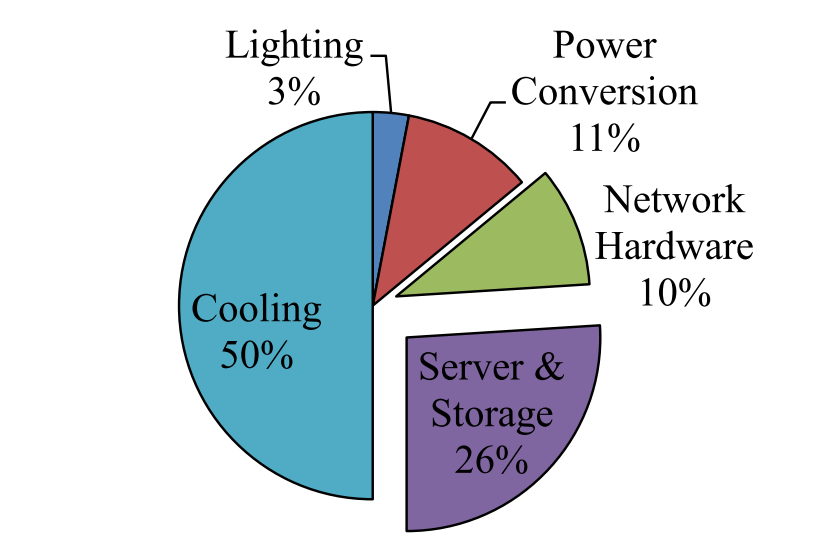
\includegraphics[width=0.7\linewidth ]{fig/energy_usage.png}
    \vspace{-2mm}
    \caption{A typical breakdown of energy usage among components in data center \cite{info2007top}.}
    \label{fig:energy_usage}
\end{figure}

\Paragraph{2. Storage space estimate from data center power usage:}
This section presents an approximate method to estimate space capacity of large social media companies like Facebook and Google.
A typical breakdown of energy consumption by data center given in Figure \ref{fig:energy_usage}.
The largest energy consuming component is cooling infrastructure with 50\% of total energy. Rest of the energy is used by power conversion, lighting, network and server components \cite{info2007top, dayarathna2016data}. Facebook data centers use efficient data center architecture and hardware tweaks  saves
8-12\% of energy spent in cooling, 13-25\% in power conversion, 10\% in motherboard \cite{frachtenberg2011high}. That implies atmost 11\%  more efficient than typical data centers. Hence, it can be claimed that Facebook servers use 37\% of energy. Considering Facebook's 138 MW Altoona data center equipped with 200 Watts servers each with $6\times4$ TB of HDD as used in their experiment for \cite{frachtenberg2011high}. Assuming the datacenter is running at peak energy $(138 \times 0.37 \times 24)/ 200 = 6127200$  TB $= 6.1272$ exabytes (EB).
Taking all the data centers in consideration and diving them with replication factor we can estimate the storage capacity of Facebook. The analysis provided above supports news {\em Facebook Builds Exabyte Data Centers for Cold Storage} in 2013 \cite{facebook_support}.


\subsection*{Social Media Data for Researchers:}
Regardless of the vast data in social media sites. the dataset availables for researchers in public domain is very very limited. Also these datasets size are miniscule in comparison to what we mean by bigdata. The only exception is Twitter. Twitter provides $\tilde 1\%$ of sample tweets through its streaming API. By utilizing multiple resources and some other APIs such as keyword search researchers can obtain more than 1\% sample data. Also it is noteworthy that researchers looking for geotagged data face greater challenge as only 0.85\% of tweets in Twitter are geotagged \cite{sloan2013knowing}. A study on the sample tweets and orginial stream (firehose) reveals that the research on sample and original can differ unless proper coverage is taken care of during data collection strategy  \cite{morstatter2013sample}. From the previous analysis and checking our twitter streaming collection, we can estimate that $\tilde 1\%$ sample collects 25-30 GB of uncompressed data daily.

Facebook has tighten the security and restricted access to many of its data for public research after Cambridge Analytical Scandal \cite{cambridge_analytica, fb_data}. However, Facebook launched an initiative to make a dataset available to {\em The Social Science Research Council} for assessment on impact of social data on election \cite{fb_initiative}. That means only affiliated researchers with certain agencies will be able to access Facebook's data. I believe we will continue to see restrict access behavior from similar social media sites in future which can affect public researchers.

To sum up, I present some of the most relevant social media dataset available for public research in Table \ref{table:datasets}. From the Table \ref{table:datasets} it is clear that there is no relationship between the amount of data social media sites possesses and the data available for researchers in public domain.

Many social media sites expose APIs for developers to access data. The free APIs of all the relevant social media sides are very restrictive. For example, facebook allows 200 api requests per hours/user. Instagram earlier had 5000 requests/hour which has been reduced to 200 request/hour. Geolocation service like foursquare 500 requests/hour on premium api end points. Hence, it is clear that availability of social media data in public domain is not only subject to effort we invest in collecting it but also restrictive policies from companies. We will revisit about scraping challanges in next section.

\begin{table}[t]
  \vspace{5mm}
      \caption{Most relevant social media dataset. }
      \vspace{-3mm}
{\small
\centering
    \begin{adjustbox}{width=1.05\linewidth,center}
\begin{tabular}{|l | l | r | l |} \hline
   \textbf{Site}                         & \textbf{Dataset}     & \textbf{Size} & \textbf{Link}  \\ \hline

   \multirow{5}{*}{\begin{tabular}{@{}l@{}} \href{http://networkrepository.com/}{Network Repository} \end{tabular}} &    Frienster      & \multicolumn{1}{r|}{8 GB} &  \href{http://networkrepository.com/soc-friendster.php}{link}   \\  \cline{2-4}

               & Twitter (1)      & \multicolumn{1}{r|}{6 GB} &  \href{http://networkrepository.com/soc-twitter-mpi-sws.php}{link}  \\\cline{2-4}

               & Twitter (2)      & \multicolumn{1}{r|}{6 GB} &  \href{http://networkrepository.com/soc-twitter.php}{link}  \\\cline{2-4}

               & Twitter (3)      & \multicolumn{1}{r|}{960 MB} &  \href{http://networkrepository.com/soc-twitter-2010.php}{link}  \\\cline{2-4}

               & Orkut (1)     & \multicolumn{1}{r|}{388 MB} &  \href{http://networkrepository.com/soc-orkut.php}{link}  \\\cline{2-4}

               & Orkut (2)     & \multicolumn{1}{r|}{422 MB} &  \href{http://networkrepository.com/soc-orkut-dir.php}{link}  \\\cline{2-4}


               & Sina Weibo      & \multicolumn{1}{r|}{960 MB} &  \href{http://networkrepository.com/soc-sinaweibo.php}{link}  \\\cline{1-4}

     \multirow{5}{*}{\begin{tabular}{@{}l@{}} \href{https://snap.stanford.edu/data/}{Stanford SNAP} \end{tabular}} &    Facebook (ego)      & \multicolumn{1}{r|}{4,039 nodes} &  \href{http://snap.stanford.edu/data/ego-Facebook.html}{link}   \\  \cline{2-4}

                 & Google Plus      & \multicolumn{1}{r|}{107,614 nodes} &  \href{http://snap.stanford.edu/data/ego-Gplus.html}{link}  \\\cline{2-4}

                 & Twitter Social      & \multicolumn{1}{r|}{81,306 nodes} &  \href{http://snap.stanford.edu/data/ego-Twitter.html}{link}  \\\cline{2-4}

                 & Expinion      & \multicolumn{1}{r|}{75,879 nodes} &  \href{http://snap.stanford.edu/data/soc-Epinions1.html}{link}  \\\cline{2-4}

                 & Youtube     & \multicolumn{1}{r|}{1,134,890 nodes} &  \href{http://snap.stanford.edu/data/com-Youtube.html}{link}  \\\cline{2-4}

                 & Amazon Product     & \multicolumn{1}{r|}{334,863	 nodes} &  \href{http://snap.stanford.edu/data/com-Amazon.html}{link}  \\\cline{2-4}

                 & Reddit     & \multicolumn{1}{r|}{132,308 submissions} &  \href{http://snap.stanford.edu/data/web-Reddit.html}{link}  \\\cline{2-4}

                & Flickr     & \multicolumn{1}{r|}{2,316,948 images} &  \href{http://snap.stanford.edu/data/web-flickr.html}{link}  \\\cline{2-4}


                & BrightKite (Location)     & \multicolumn{1}{r|}{58,228 Nodes} &  \href{http://snap.stanford.edu/data/loc-Brightkite.html}{link}  \\\cline{2-4}

                 & Gowalla (Location)     & \multicolumn{1}{r|}{196,591 Nodes} &  \href{http://snap.stanford.edu/data/loc-Gowalla.html}{link}  \\\cline{2-4}

                 & Movies & \multicolumn{1}{r|}{196,591 Nodes} &  \href{http://snap.stanford.edu/data/web-Movies.html}{link} \\\cline{1-4}

     \multirow{5}{*}{\begin{tabular}{@{}l@{}} \href{http://socialcomputing.asu.edu/pages/datasets}{Social Computing ASU} \end{tabular}} &    Youtube (1)      & \multicolumn{1}{r|}{1,138,499 nodes} &  \href{http://socialcomputing.asu.edu/datasets/YouTube2}{link}   \\  \cline{2-4}

                 & Youtube (2)      & \multicolumn{1}{r|}{15088 nodes} &  \href{http://socialcomputing.asu.edu/datasets/YouTube}{link}  \\\cline{2-4}

                 & Last FM      & \multicolumn{1}{r|}{108,493 nodes} &  \href{http://socialcomputing.asu.edu/datasets/Last.fm}{link}  \\\cline{2-4}

                 & Twitter      & \multicolumn{1}{r|}{11,316,811 tweets} &  \href{http://socialcomputing.asu.edu/datasets/Twitter}{link}  \\\cline{2-4}

                 & Flickr      & \multicolumn{1}{r|}{80,513 nodes} &  \href{http://socialcomputing.asu.edu/datasets/Flickr}{link}  \\\cline{2-4}

                 & Foursquare     & \multicolumn{1}{r|}{106,218 nodes} &  \href{http://socialcomputing.asu.edu/datasets/Foursquare}{link}  \\\cline{2-4}

                 & Digg      & \multicolumn{1}{r|}{116,893 nodes} &  \href{http://socialcomputing.asu.edu/datasets/Digg}{link}  \\\cline{2-4}


                 & Delicious      & \multicolumn{1}{r|}{103,144 nodes} &  \href{http://socialcomputing.asu.edu/datasets/Delicious}{link}  \\\cline{1-4}

       \multirow{1}{*}{\begin{tabular}{@{}l@{}} \href{http://help.sentiment140.com/for-students}{Sentiment  140} \end{tabular}} &    Twitter Sentiment      & \multicolumn{1}{r|}{160,000 tweets} &  \href{http://help.sentiment140.com/for-students}{link}   \\  \cline{1-4}

       \multirow{1}{*}{\begin{tabular}{@{}l@{}} \href{https://www.reddit.com/r/datasets/comments/3bxlg7/i_have_every_publicly_available_reddit_comment/}{Reddit } \end{tabular}} &    Reddit     & \multicolumn{1}{r|}{1.7 billion comments} &  \href{https://www.kaggle.com/reddit/reddit-comments-may-2015}{link}   \\  \cline{1-4}

       \multirow{1}{*}{\begin{tabular}{@{}l@{}} \href{https://www.reddit.com/r/datasets/comments/3bxlg7/i_have_every_publicly_available_reddit_comment/}{Yahoo} \end{tabular}} &    Flickr      & \multicolumn{1}{r|}{100 million images} &  \href{ https://yahooresearch.tumblr.com/post/89783581601/one-hundred-million-creative-commons-flickr-images}{link}   \\  \cline{1-4}

        \multirow{2}{*}{\begin{tabular}{@{}l@{}} \href{}{Awesome Data Github} \end{tabular}} &    Google Scholar      & \multicolumn{1}{r|}{Unknown} &  \href{ http://www3.cs.stonybrook.edu/~leman/data/gscholar.db}{link}   \\  \cline{2-4}

          & Indie Map      & \multicolumn{1}{r|}{Unknown} &  \href{http://www.indiemap.org/}{link}  \\\cline{1-4}


 \end{tabular}
 \end{adjustbox}
 % \vspace{ + 15 mm}
 }
 \label{table:datasets}
 \end{table}




%%% Local Variables:
%%% mode: latex
%%% TeX-master: "main"
%%% End:

\section{Part B.}
\subsection*{Scraping Social Media:}

%%% Local Variables:
%%% mode: latex
%%% TeX-master: "main"
%%% End:


%\balance
%\vspace{-3mm}
\bibliographystyle{abbrv}
\bibliography{main}


% \vspace{-3mm}
% \bibliographystyle{ACM-Reference-Format}
% \bibliography{sigproc}

\end{document}
